\section{Sacré-Coeur}
Ačkoliv je neustále vystavována posměchu, tuto širokou daleko viditelnou baziliku připomínající šlehačkový dort si nikdo nenechá ujít. Tato bazilika postavená v novorománsko-byzantském stylu s obrovským zvonem byla v roce 1871 po prohrané válce s Německem a po porážce pařížské Komuny zamýšlena jako chrám smíření a v roce 1919 byla zasvěcena Srdci Ježíšovu. Kněží se tady dodnes ve dne v noci modlí za duše zemřelých. Na širokých schodech před vchodem lze prosedět celé hodiny a těšit se pohledu na Paříž. Interiér baziliky sice není tak impozantní jako jiné kostely ve městě, ale návštěvníky sem láká především právě panoramatická podívaná. Zvláště při západu slunce se hlouběji vryje do paměti jako jen málokterá pařížská památka.\\
\\Třpytivá mozaika Krista v byzantském stylu pochází z let 1912 – 22. vytvořil ji Luc Olivier Merson a krášlí klenbu nad kněžištěm. Vyjadřuje oddanost Francie Kristovu srdci. Nejpoutavějším prvkem interiéru je asi klenutá krypta. V jedné z kaplí je uloženo srdce Alexandra Legentila, jednoho z mecenášů Sacré-Coeur. Dveře vstupního portika dekorují nádherné bronzové reliéfy s výjevy z poslední večeře a dalšími scénami ze života Krista. Typicky vejčitá kopule baziliky je po Eiffelově veži druhou nejvyšší vyhlídkou v Paříži. Na vrchol vede točité schodiště a za jasného dne dohlédnete až do vzdálenosti 48 kilometrů. Nejvýznamnější socha v bazilice znázorňuje žehnajícího Krista. Je umístěna symbolicky v nice nad hlavním vchodem nade dvěma jezdeckými sochami.\\
\\Překrásná zvonice, kterou navrhl Lucien Magne, byla vztyčena v roce 1904 a dosahuje 80 metrů. Uvnitř je zavěšen jeden z nejtěžších zvonů na světě, devatenáctitunový La Savoyarde. Byl odlit v roce 1895 v Annecy a věnovala jej savojská diecéze. Na portiku nad hlavním vchodem se vyjímají působivé bronzové sochy francouzských světců, které odlil H. Lefébvre. Jedna představuje Janu z Arku a druhá sv. Ludvíka. Jedno z podlaží tamburu je obehnáno vitrážemi a nabízí tak úchvatný pohled na celý interiér. Architekt Paul Abadie (1875 – 1912) zakomponoval do návrhu směsici kopulí, věžiček a klasicistních prvků. Kámen ze Chateau-Landonu vylučuje, když navlhne, vápenec, který zbarvuje průčelí na bílo. Chcete-li se vyhnout výstupu do strmého kopce, využijte lanovku a cestou se kochejte pěkným výhledem. Jezdí od konce rue Foyatier poblíž place Willette\index{Willette}.

\begin{figure}[h!]
\centering
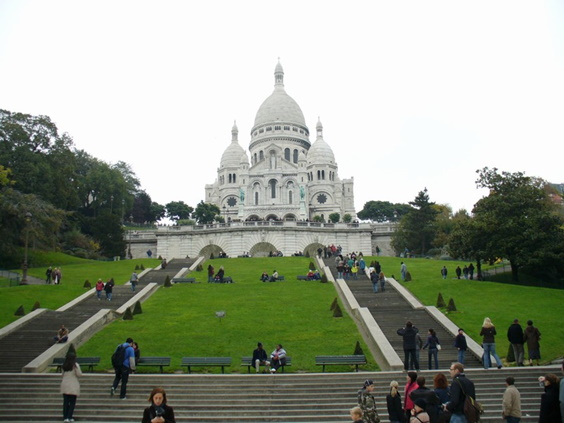
\includegraphics[scale=0.5]{images/obr5S.jpg}
\caption{Sacré-Coeur}

\end{figure}

\section{Katedrála Notre-Dame}
Tato katedrála Matky Boží je symbolem Paříže a jednou z nejvýznamnějších sakrálních staveb rané gotiky. Tady, v srdci města, kdysi stála raně křesťanská bazilika, potom románský kostel. V roce 1163 dal Maurice de Sully, biskup pařížský, zahájit stavbu, která byla dokončena v roce 1345. Od té doby byla Notre-Dame dějištěm celé řady královských slavností: v roce 1430 zde byl korunován Jindřich VI. anglickým králem Francie, v roce 1559 tu proběhla korunovace Marie\index{Marie} Stuartovny. Za Francouzské revoluce prohlásil Robespierre tuto katedrálu „chrámem rozumu“. V roce 1804 tvořila kulisu k císařské korunovaci Napleona za přítomnosti papeže. Těžké škody vzniklé v důsledku revoluce odstranil v roce 1844 Viollet-le-Duc.\cite{cada}\\
\begin{figure}[h!]
\centering
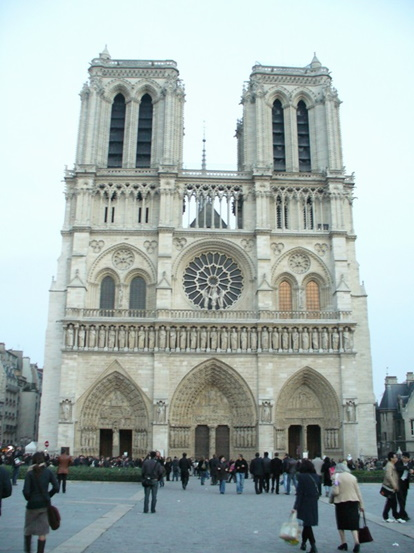
\includegraphics[scale=0.5]{images/obr6N.jpg}
\caption{Katedrála Notre-Dame}

\end{figure}\\Do katedrály lze vstoupit třemi portály s úchvatnou reliéfní výzdobou. Středověké biblické výjevy líčí život Panny Marie\index{Marie}, poslední soud a život sv. Anny. Nad nimi uvidíte galerii judských a izraelských králů. Nádherný tympanon byl ztvárněn ve 13. století a zachycuje smrt Panny Marie\index{Marie} a její slavností korunovaci v nebi. Sousoší Panny Marie\index{Marie} s dítětem na dveřním pilíři je však moderní. Slavná je dokonale krásná gotická fasáda se třemi portály a královskou galerií. Umělecky zpracovaná růžice pod arkádami Velké galerie měří v průměru deset metrů.\\\\Výhled z věže je odměnou za opravdu namáhavý výstup   věže totiž měří 69 metrů a mají 387 schodů. Návštěvníci se mohou jít podívat do té severní, v jižní je totiž zvon zvaný Emanuel vážící 13 tun. Působivý opěrný systém, podepírající východní závěr katedrály, je dílem Jeana Ravyho a má rozpětí 15 metrů. Nejlépe jej lze obdivovat z náměstí Place Jean XXIII. Mezi věžemi jsou ukryty legendární chrliče (chimiéres), jež sem umístil Viollet-le-Duc, aby odvracely zlo.\\\\Severní, jižní a západní průčelí krášlí tři skvostná rozetová okna. Vitráž\index{vitráž} s Pannou Marií obklopenou postavami ze Starého zákona z 13. století si však zachovalo pouze severní průčelí. Jižní rozetové okno vyobrazuje Krista mezi apoštoly. Více než polovina původních lavic v katedrále, které nechal zhotovit Ludvík XIV.\index{Ludvík XIV.}, se dochovala. Překrásná dřevořezba zachycuje také výjevy ze života Panny Marie\index{Marie}. U vchodu do kněžiště, naproti jihovýchodnímu pilíři transeptu, najdeme nádhernou sochu ze 14. století. Je známá jako Notre-Dame de Paris (Panna Marie\index{Marie} Pařížská) a byla sem přemístěna z kaple sv. Aignana. Sakristie uchovává staré rukopisy, relikviáře a církevní roucha. Trnová koruna a fragmenty pravého Kříže může veřejnost obdivovat vždy na Velký pátek.\cite{pecinovsky}
\begin{figure}[h!]
\centering
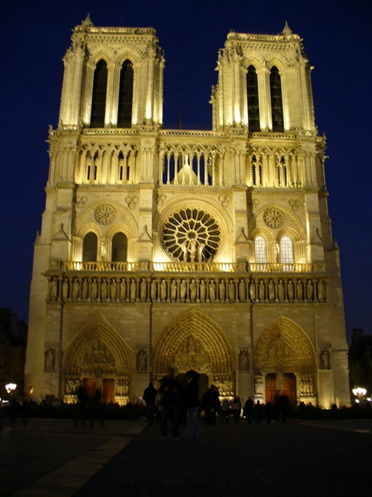
\includegraphics[scale=0.5]{images/obr7N.jpg}
\caption{Osvětlená Notre-Dame}

\end{figure}
